\documentclass[11pt]{article}
\usepackage{acl2014}
\usepackage{times}
\usepackage{url}
\usepackage{latexsym}
\usepackage{helvet}
\usepackage{courier}
\usepackage{latexsym}
\usepackage{amsmath}
\usepackage{multirow}
\usepackage{graphicx}
\usepackage{subfigure}
\usepackage{relsize}
\usepackage{hhline}
\usepackage[usenames]{color}
\usepackage{colortbl,booktabs}
%\usepackage{slashbox}
\usepackage{balance}
\usepackage{xcolor}
\usepackage{amsmath}
\usepackage{color}
\usepackage{multirow}
\usepackage{wrapfig}
\usepackage{algorithm}
\usepackage{tabularx}
\usepackage{url}
\usepackage{algpseudocode}
\definecolor{mygray}{gray}{.5}

\renewcommand{\baselinestretch}{0.95}

%\setlength\titlebox{5cm}

% You can expand the titlebox if you need extra space
% to show all the authors. Please do not make the titlebox
% smaller than 5cm (the original size); we will check this
% in the camera-ready version and ask you to change it back.


% Alternate titles.

\title{Are Two Heads Better than One? Crowdsourced Translation via a \\Two-Step Collaboration of Non-Professional Translators and Editors}

\author{Rui Yan, Mingkun Gao, Ellie Pavlick, and Chris Callison-Burch \\
Computer and Information Science Department, \\
University of Pennsylvania, Philadelphia, PA, U.S.A.\\
\normalsize{{\tt \{ruiyan,gmingkun,epavlick\}@seas.upenn.edu, ccb@cis.upenn.edu}}}

\date{}

\begin{document}
\maketitle
\begin{abstract}
  Crowdsourcing is a viable mechanism for creating training data for machine translation.  It provides a low cost, fast turn-around way of processing large volumes of data. However, when compared to professional translation, naive collection of translations from non-professionals yields low-quality results. Careful quality control is necessary for crowdsourcing to work well. In this paper, we examine the challenges of a two-step collaboration process with translation and post-editing by non-professionals.  We develop graph-based ranking models that automatically select the best output from multiple redundant versions of translations and edits, and improves translation quality closer to professionals.
\end{abstract}

\section{Introduction}

Statistical machine translation (SMT) systems are trained using bilingual sentence-aligned parallel corpora.  Theoretically, SMT can be applied to any language pair, but in practice it produces the state-of-art results only for language pairs with ample training data, like English-Arabic, English-Chinese, French-English, etc.  SMT gets stuck in a severe bottleneck for many minority or `low resource' languages with insufficient data.
This drastically limits which languages SMT can be successfully applied to.
Because of this, collecting parallel corpora for minor languages has become an interesting research challenge. There are various options for creating training data for new language pairs.  Past approaches have examined harvesting translated documents from the web \cite{a10,a13,smith-EtAl:2013:ACL}, or discovering parallel fragments from comparable corpora \cite{a11,abdulrauf-schwenk:2009:EACL,a12}.
Until relatively recently, little consideration has been given to creating parallel data from scratch.  This is because the cost of hiring professional translators is prohibitively high.  For instance, \newcite{a25} hoped to hire professional translators to create a modest sized 100,000 word Tamil-English parallel corpus, but were stymied by the costs and the difficulty of finding good translators for a short-term commitment.

Recently, crowdsourcing has opened the possibility of translating large amounts of text at low cost using non-professional translators.  Facebook localized its web site into different languages using volunteers \cite{Facebook-Crowdsourced-Translation}.  DuoLingo turns translation into an educational game, and translates web content using its language learners \cite{vonAhn:2013:DLL:2449396.2449398}.
%Crowdsourcing translation research in the NLP community has focused on hiring workers on the Amazon Mechanical Turk platform   \cite{Callison-Burch2009}, rather than relying on volunteers or gamification.
Rather than relying on volunteers or gamification, NLP research into crowdsourcing translation has focused on hiring workers on the Amazon Mechanical Turk  (MTurk) platform   \cite{Callison-Burch2009}.  This setup presents unique challenges, since it typically involves non-professional translators whose language skills are varied, and since it sometimes involves participants who try to cheat to get the small financial reward \cite{zaidan-callisonburch:2011:ACL-HLT2011a}.
A natural approach for trying to shore up the skills of weak bilinguals is to pair them with a native speaker of the target language to edit their translations.
We review relevant research from NLP and human-computer interaction (HCI) on collaborative translation processes in Section \ref{related-work}.
To sort good translations from bad, researchers often solicit multiple, redundant translations and then build models to try to predict which translations are the best, or which translators tend to produce the highest quality translations.

The contributions of this paper are:
\begin{itemize}
\item An analysis of the difficulties posed by a two-step collaboration between editors and translators in Mechanical Turk-style crowdsourcing environments.  Editors vary in quality, and poor editing can be difficult to detect.
\item A new graph-based algorithm for selecting the best translation among multiple translations of the same input.  This method takes into account the collaborative relationship between the translators and the editors.
\end{itemize}
%
% conducted a preliminary study that compared the quality of professional translators to non-professional translators hired on Amazon Mechanical Turk (MTurk) for translations from Spanish, German, French, Chinese into Urdu.  \newcite{zaidan-callisonburch:2011:ACL-HLT2011a}
%
%More recent efforts have used crowdsourcing to create
%%
%
%A worthy effort would be seeking for higher quality translations at a lower cost. We notice that Amazon's Mechanical Turk (MTurk) provides a labor force platform at a cheap price for labor units, and hence we are able to hire a large group of translators, non-professional or even professional, at a similarly tempting low price. In the way of crowdsourcing, we could manage to create a large parallel corpus at a fraction of the cost of professional translators. With affordable human computation achieved, we aim at soliciting high quality translations out of the redundant, perhaps low-quality, disfluent generations. We have proposed a random walk of mutual reinforced ranking model based on a heterogenous graph consisting of translations and the workers on MTurk, named MTurkers. In particularly, we design a schema of collaborative crowdsourcing: translation followed by post-editing. We also include linguistic quality scoring as the ranking prior during the selection process. After these two steps, the collaboration of two non-professional generate a translated sentence. The model discriminates acceptable translations from those that are not (and analogously competent Turkers from those who are not).
%
%According to an objective and quantitative comparison with the professionally-produced reference translations as a weights set, we examine the idea of enabling the 2-step of ``\textit{collaborations}'' between both roles of non-professional translators and post-editors, and using structural information from the collaboration relationships. We show that it is possible to get near professional high quality translations in aggregate by soliciting multiple translations to select the best of the bunch (and the cost can be even lower to identifying competent MTurkers). The overall performance is improved by the 2-step collaboration and the information hidden in the net structure: in other words, \textbf{TWO} heads are indeed better than \textbf{ONE}.
%
%
%We start by introducing the crowdsourcing platform and data collection. In Section 3 we formulate a reinforced ranking model combined with random walk, and then describe experimental results in Section 4. We review related work in Section 5 and draw conclusions in Section 6.
%
%
%\section{Crowdsourcing Platform and Data Collection}
%To collect crowdsourced translations, we deploy our platform based on Amazon's Mechanical Turk, an online market-place designed to pay people small sums of money to complete \textit{Human Intelligence Tasks} (or HIT) � tasks that are difficult for computers but easy for people. Example HIT ranges from labeling images or annotating texts and semantics to providing feedback on relevance of results for search queries \cite{zaidan-callisonburch:2011:ACL-HLT2011a}. Anyone with an Amazon account can either submit HIT or work on HIT that were submitted by others. Workers are referred to as ``Turkers'', and designers of HIT as ``Requesters''. A Requester specifies the reward to be paid for each completed item. The relationship between Turkers and Requesters is designed to be a mutual selection: Turkers are free to select whichever HIT interests them, and requesters can choose not to pay for unsatisfied results.
%
%The advantages of Mechanical Turk are obvious: zero overhead for hiring workers with a large, low-cost labor force and the task can be completed in a naturally parallel pattern by vast individuals so that the turnaround time is short. For Natural Language Processing, it is easier to access to foreign markets with native speakers of many rare languages. On the other hands, the Turkers are completely anonymous without any personal profile other than a Turker ID (eg., A143AWKU99STC9). Hence it is difficult to determine if a non-professional is qualified to fulfill the task before the Turker submits HIT.
%
%In this sense, soliciting translations from anonymous non-professionals carries a significant risk of poor translation quality, but it is not very difficult to find bad translations provided by Turkers using simple linear regression methods \cite{zaidan-callisonburch:2011:ACL-HLT2011a}. To improve the accuracy of noisy translations from non-experts, a natural quality control solution would be employing a graph-based ranking model to quantitatively measure multiple outputs based on ``votes'' or ``recommendations'' between each other, namely the wisdom of crowds.
%

\section{Related work}\label{related-work}



In the HCI community, several researchers have proposed protocols for collaborative translation efforts \cite{Morita:2009:PRIMA,Morita:2009:IUI,Hu:2009,Hu:2010}.  These have focused on an iterative collaboration between monolingual speakers of the two languages, facilitated with a machine translation system.
%plus additional communication channels, like the ability to annotate portions of the text with Wikipedia links or images.
These studies are similar to ours in that they rely on native speakers' understanding of the target language to correct the disfluencies in poor translations.  In our setup the poor translations are produced by bilingual individuals who are weak in the target language, and in their experiments the translations are the output of a machine translation system.\footnote{A variety of HCI and NLP studies have confirmed the efficacy of monolingual or bilingual individuals post-editing of machine translation output \cite{callisonburch:2005:NIST,koehn:2010:NAACLHLT,Green:2013:EHP:2470654.2470718}.  Past NLP work has also examined automatic post-editing\cite{Knight94automatedpostediting}.}
%The same improvements would presumably result when native speakers of the target language edit translations produced by  (which is the case in our setup).
Another significant difference is that the HCI studies assume cooperative participants.   For instance, \newcite{Hu:2010} recruited volunteers from the International Children's Digital Library \cite{hourcade2003international} who were all well intentioned and participated out a sense of altruism and to build a good reputation among the other volunteer translators at \url{childrenslibrary.org}.
Our setup uses anonymous crowd workers hired on Mechanical Turk, whose motivation to participate is financial.
%
\newcite{bernstein-et-al:2010} characterized the problems with hiring editors via MTurk for a word processing application.  Workers were either lazy (meaning they made only minimal edits) or overly zealous (meaning they made many unnecessary edits).  \newcite{bernstein-et-al:2010} addressed this problem with a three step find-fix-verify process.  In the first step, workers click on one word or phrase that needed to be corrected.  In the next step, a separate group of workers proposed corrections to problematic regions that had been identified by multiple workers in the first pass.  In the final step, other workers would validate whether the proposed corrections were good.

Most NLP research into crowdsourcing has focused on Mechanical Turk, following pioneering work by \newcite{Snow-et-al:EMNLP:2008} who showed that the platform was a viable way of collecting data for a wide variety of NLP tasks at low cost and in large volumes.  They further showed that non-expert annotations are similar to expert annotations when many non-expert labelings for the same input are aggregated, through simple voting or through weighting votes based on how closely non-experts matched experts on a small amount of calibration data.  MTurk has subsequently been widely adopted by the NLP community and used for an extensive range of speech and language applications \cite{callisonburch-dredze:2010:MTURK}.

Although hiring professional translators to create bilingual training data for machine translation systems has been deemed infeasible, Mechanical Turk has provided a low cost way of creating large volumes of translations \cite{Callison-Burch2009,ambati:10}.  For instance,  \newcite{Zbib-etal:2012:NAACL,zbib-EtAl:2013:NAACL-HLT} translated 1.5 million words of Levine Arabic and Egyptian Arabic, and showed that a statistical translation system trained on the dialect data outperformed a system trained on 100 times more MSA data.  \newcite{post-callisonburch-osborne:2012:WMT} used MTurk to create parallel corpora for six Indian languages for less than \$0.01 per word.  MTurk workers translated more than half a million words worth of Malayalam in less than a week.  Several researchers have examined the use of active learning to further reduce the cost of translation \cite{a7,AmbatiThesis,bloodgood-callisonburch:2010:ACL}.  Crowdsourcing allowed real studies to be conducted whereas most past active learning were simulated. \newcite{Pavlick:2014} conducted a large-scale demographic study of the languages spoken by workers on MTurk by translating 10,000 words in each of 100 languages.  \newcite{chen:2011}  examined the steps necessary to build a persistent multilingual workforce on MTurk.

This paper is most closely related to previous work by \newcite{zaidan-callisonburch:2011:ACL-HLT2011a}, who showed that non-professional translators could approach the level of professional translators.  They solicited multiple redundant translations from different Turkers for a collection of Urdu sentences that had been previously professionally translated by the Linguistics Data Consortium.  They built a model to try to predict on a sentence-by-sentence and Turker-by-Turker which was the best translation or translator.  They also hired US-based Turkers to edit the translations, since the translators were largely based in Pakistan and exhibited errors that are characteristic of speakers of English as a language. \newcite{zaidan-callisonburch:2011:ACL-HLT2011a} observed only modest improvements when incorporating these edited translation into their model.  We attempt to analyze why this is, and we proposed a new model to try to better leverage their data.


\begin{table}[t]
\centering
\begin{tabular}{|l|} \hline
Urdu translator:\\ \hline
 \begin{minipage}[position]{0.45\textwidth}
  \vspace{1mm}\small{According to the territory's people the pamphlets from the Taaliban had been read in the announcements in all the mosques of the Northern Wazeerastan.}\vspace{1mm}
 \end{minipage}
\\ \hline \end{tabular}
\begin{tabular}{|l|} \hline
English post-editor:\\ \hline
 \begin{minipage}[position]{0.45\textwidth}
    \vspace{1mm}\small{According to locals, the pamphlet released by the Taliban was read out on the loudspeakers of all the mosques in North Waziristan.}\vspace{1mm}
 \end{minipage}
\\ \hline \end{tabular}
\begin{tabular}{|l|} \hline
LDC professional:\\ \hline
 \begin{minipage}[position]{0.45\textwidth}
      \vspace{1mm}\small{According to the local people, the Taliban's pamphlet was read over the loudspeakers of all mosques in North Waziristan.} \vspace{1mm}
 \end{minipage}
\\ \hline \end{tabular}
\caption{Different versions of translations.}
\label{translations}
\end{table}


%{\sc todo - cite past work on crowdsourcing translation \nocite{*}}
\nocite{*}


\section{Crowdsourcing Translation}


\paragraph{Setup}

We conduct our experiments using the data collected by \newcite{zaidan-callisonburch:2011:ACL-HLT2011a}. This data set consists 1,792 Urdu sentences from a variety of news and online sources, each paired with English translations provided by non-professional translators on Mechanical Turk. 

Each Urdu sentence was translated redundantly by 3 distinct translators, and each translation was edited by 3 separate (native English-speaking) editors to correct for grammatical and stylistic errors. In total, this gives us 12 non-professional English candidate sentences (3 unedited, 9 edited) per original Urdu sentence. 52 different Turkers took part in the translation task, each translating 138 sentences on average. In the editing task, 320 Turkers participated, averaging 56 sentences each. For comparison, the data also includes 4 different reference translations for each source sentence, produced by professional translators. 

Table \ref{translations} gives an example of an unedited translation, an edited translation, and a professional translation for the same sentence. The translations provided by translators on MTurk are generally done conscientiously, preserving the meaning of the source sentence, but typically contain simple mistakes like misspellings, typos, and awkward word choice. English-speaking editors, despite having no knowledge of the source language, are able to fix these errors. In this work, we show that the collaboration design of two heads-- non-professional Urdu translators and non-professional English editors-- yields better translated output than would either one working in isolation, and can better approximate the quality of professional translators. 


%\subsection{One-Step Model}
%\subsection{Two-Step Collaboration Model}

%\begin{table}[t]
%\centering
%\begin{tabular}{|p{\linewidth}|} \hline
%Urdu translator:\\ \hline
%\small{According to the territory's people the pamphlets from the Taaliban had been read in the announcements in all the mosques of the Northern Wazeerastan.}\\\hline
%English post-editor:\\ \hline
%\small{According to locals, the pamphlet released by the Taliban was read out on the loudspeakers of all the mosques in North Waziristan.}\\\hline
%LDC professional:\\ \hline
%\small{According to the local people, the Taliban's pamphlet was read over the loudspeakers of all mosques in North Waziristan.} \\\hline
%\end{tabular}
%\caption{Different versions of translations.}
%\label{translations}
%\end{table}


\paragraph{Analysis}

We know from inspection that translations seem to improve with editing (Table \ref{translations}). Given the data from MTurk, we explore whether this is the case in general: Do all translations improve with editing? To what extent does the individual translator and the individual editor effect the quality of the final sentence?

\begin{figure}[h]
  \centering
  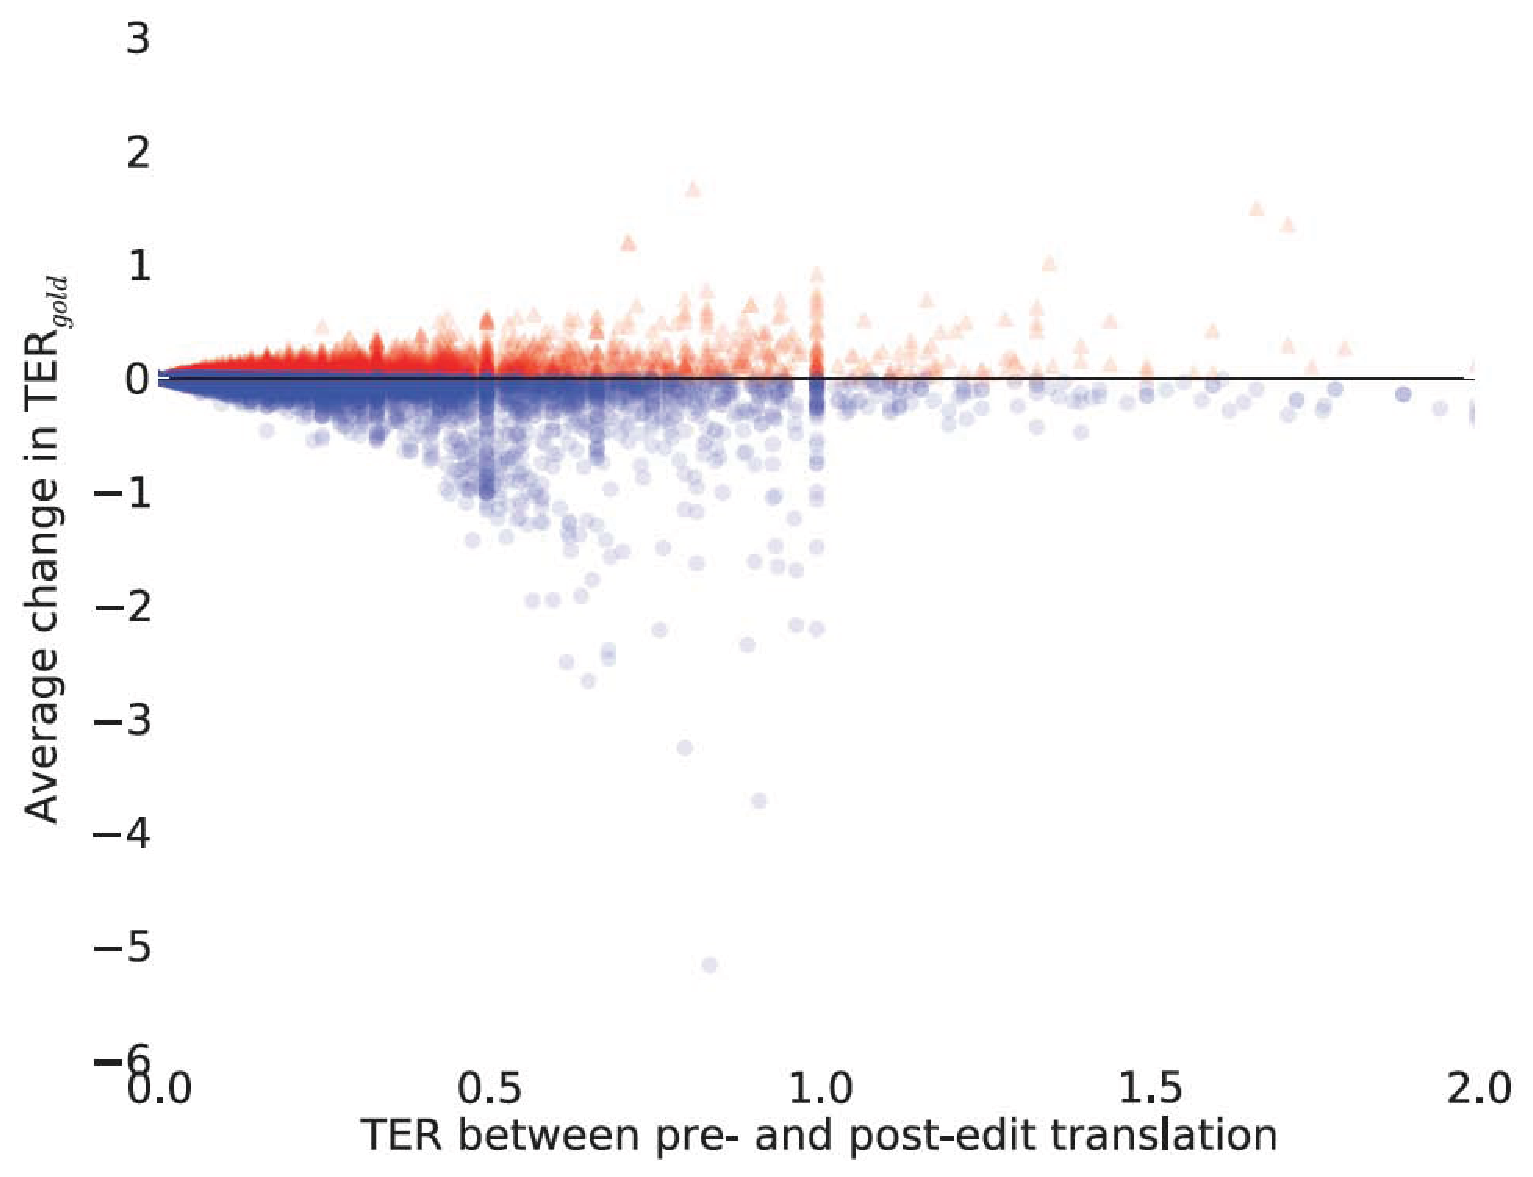
\includegraphics[width=\linewidth]{translation-editor-scatter}
  \caption{Relationship between editor aggressiveness and effectiveness. Each point represents an editor/translation pair. Aggressiveness (x-axis) is measured as the TER between the pre-edit and post-edit version of the translation, and effectiveness (y-axis) is measured as the average amount by which the editing reduces the translation's TER$_{gold}$. While many editors make only a few changes, those who make many changes can bring the translation substantially closer to professional quality.}
    \label{editor-scatter}
\end{figure}

\begin{figure}[h]
  \centering
  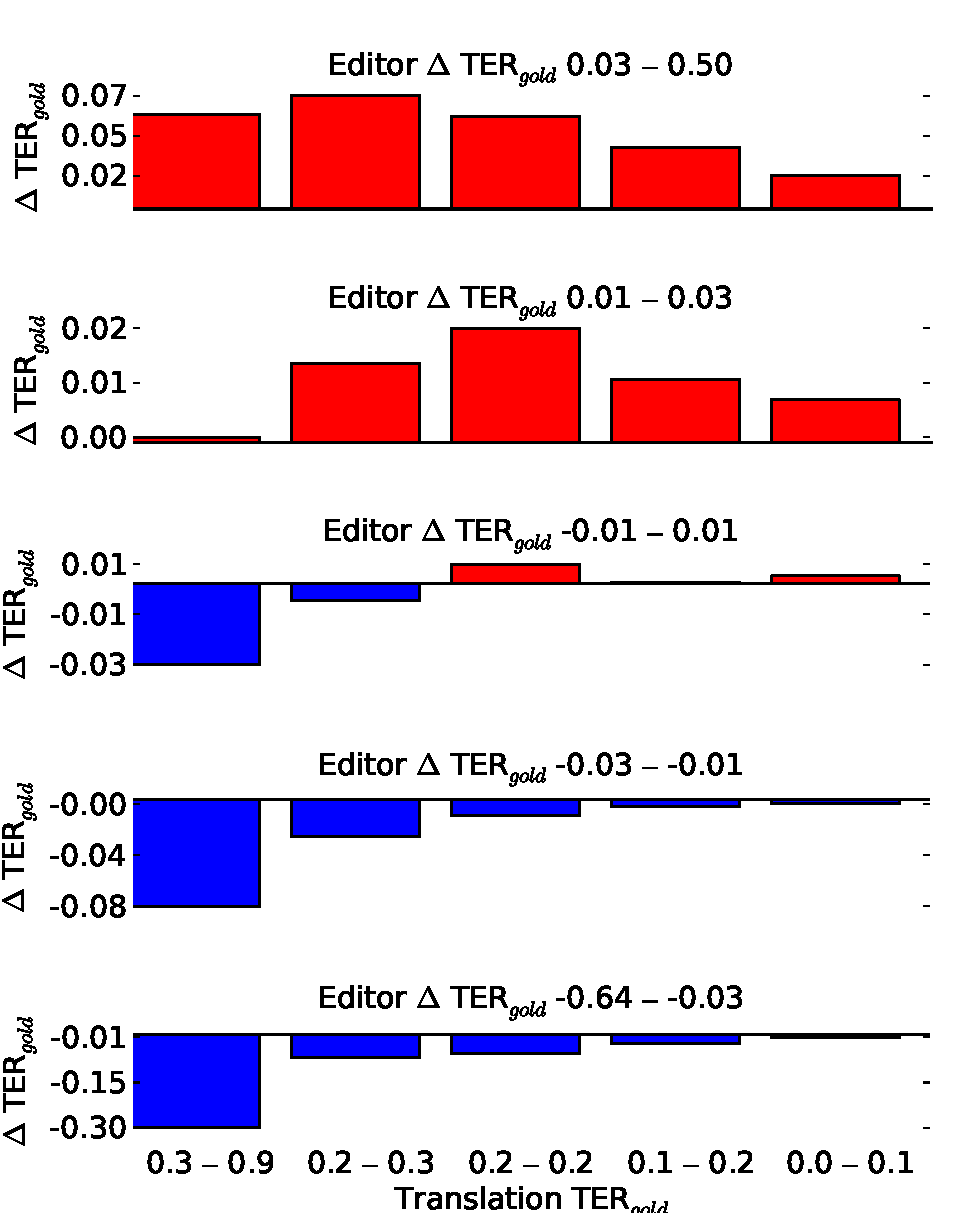
\includegraphics[width=\linewidth]{editor-bins}
  \caption{Effect of editing on translations of varying quality. Rows reflect bins of editors, with the worse editors (those whose changes result in increased TER$_{gold}$) on the top and the most effective editors (those whose changes result in the largest reduction in TER$_{gold}$) on the bottom. Bars reflect bins of translations, with the highest TER$_{gold}$ translations on the left, and the lowest on the right. We can see from the consistently negative $\Delta$ TER$_{gold}$ in the bottom row that good editors are able to improve both good and bad translations.}
    \label{editor-bins}
\end{figure}


We use \textit{translation edit rate} (TER) as a measure of translation similarity. TER represents the amount of change necessary to transform one sentence into another, so a low TER means the two sentences are very similar. To capture the quality (``professionalness'') of a translation, we take the average TER of the translation against each of our gold translations. That is, we define TER$_{gold}$ of translation $t$ as

\begin{align}
TER_{gold} = \frac{1}{4}\sum\limits_{i = 1}^4 TER(gold_i, t)
\end{align}

where a lower TER$_{gold}$ is indicative of a higher quality (more professional-sounding) translation.


We first look at editors along two dimensions: their aggressiveness and their effectiveness. Some editors may be very aggressive (they make many changes to the original translation) but still be ineffective (they fail to bring the quality of the translation closer to that of a professional). We measure aggressiveness by looking at the TER between the pre- and post-edited versions of each editor's translations; higher TER implies more aggressive editing. To measure effectiveness, we look at the change in TER$_{gold}$ that results from the editing; negative $\Delta$TER$_{gold}$ means the editor effectively improved the quality of the translation, while positive $\Delta$TER$_{gold}$ means the editing actually brought the translation further from our gold standard.


Figure \ref{editor-scatter} shows the relationship between these two qualities for individual editor/translation pairs. We see that while most translations require only a few edits, there are a large number of translations which improve substantially after heavy editing. This trend conforms to our intuition that editing is most useful when the translation has much room for improvement, and opens the question of whether good editors can offer improvements to translations of all qualities.

\begin{figure*}[ht!]
  \centering
  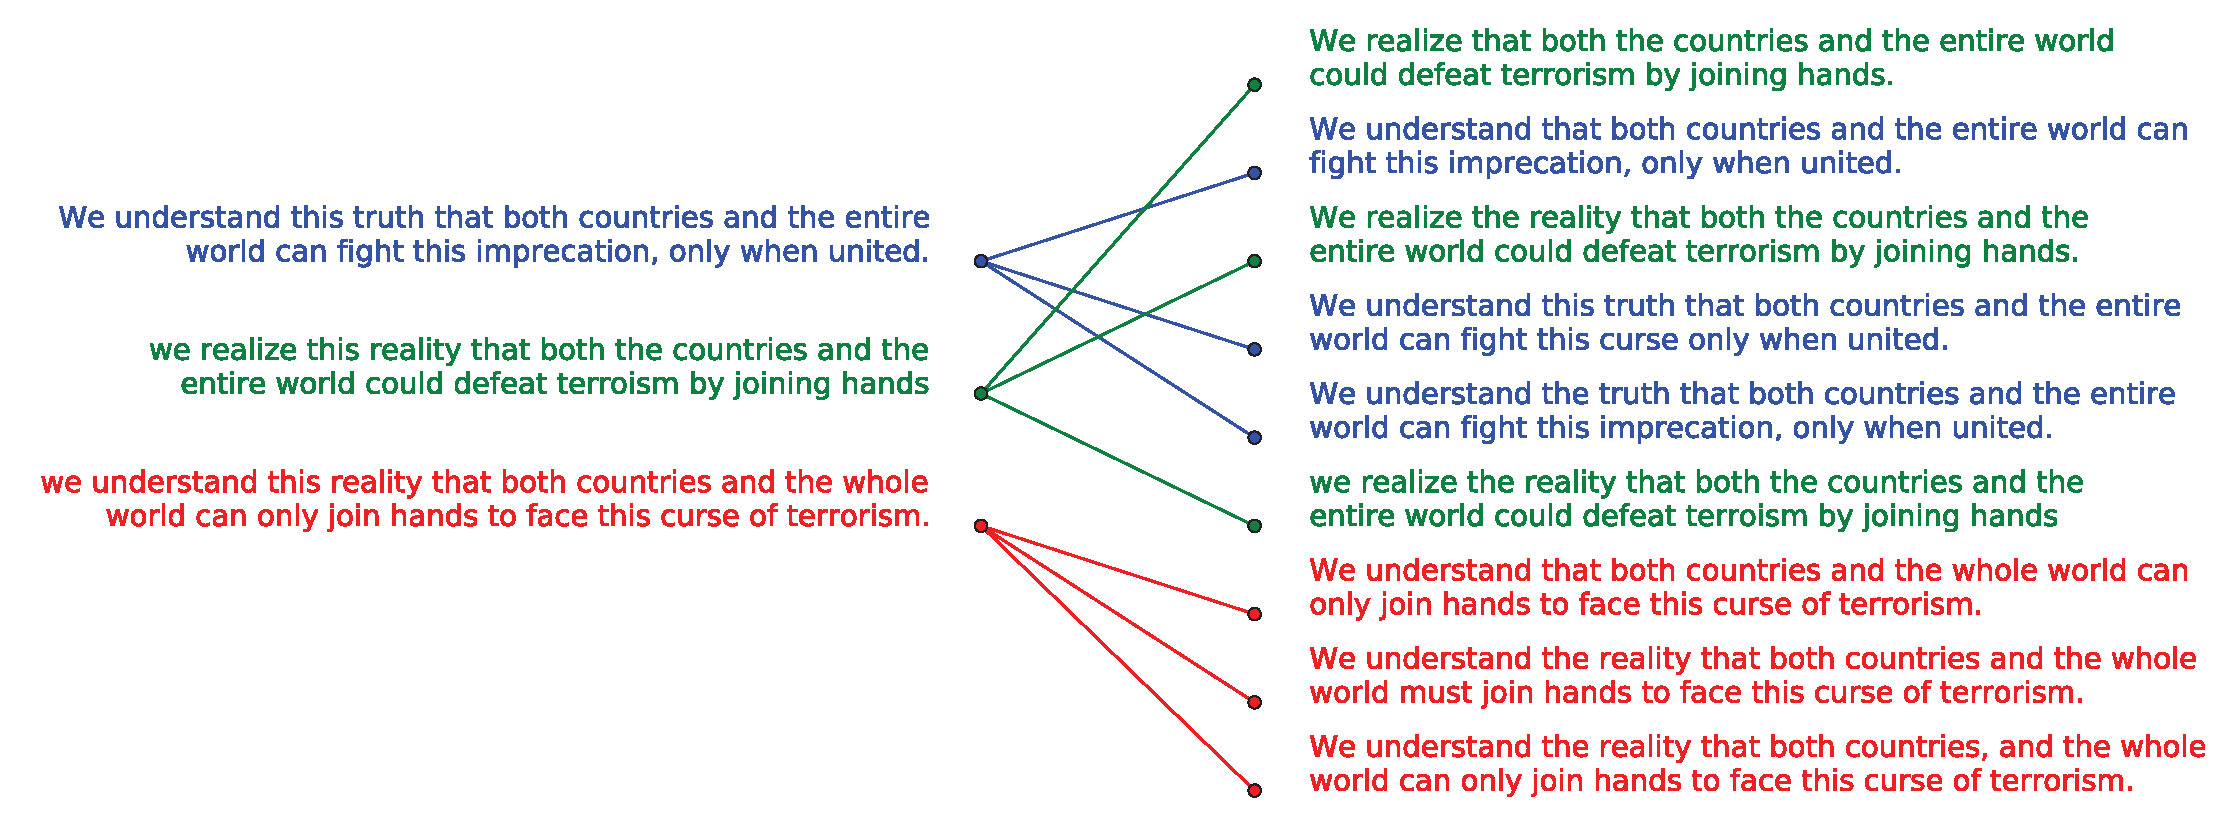
\includegraphics[width=\linewidth]{ter-rerank}
  \caption{Three alternative translations (left) and the edited versions of each (right). Each edit on the right was produced by a different editor. Order reflects the TER$_{gold}$ of each translation, with the lowest TER$_{gold}$ on the top. Some translators receive low TER$_{gold}$ scores due to superficial errors, which can be easily improved through editing. In the above example, the middle-ranked translation (green) becomes the best translation after being revised by a good editor.}
    \label{rerank}
\end{figure*}

To address this question, we split our translations into 5 bins, based on their TER$_{gold}$.  We also split our editors into 5 bins, based on their effectiveness (i.e. the average amount by which their editing reduces TER$_{gold}$). Figure \ref{editor-bins} shows the degree to which editors at each level are able to improve the translations from each bin. We see that good editors are able to make improvements to translations of all qualities, but that good editing has the greatest impact on lower quality translations. This result suggests that finding good editor/translator pairs, rather than good editors and good translators in isolation, should produce the best translations overall. Figure \ref{rerank} gives an example of how an initially medium-quality translation, when combined with good editing, produces a better result than the higher-quality translation paired with mediocre editing.


%Figure 1 gives more typical translation examples.

\section{Problem Formulation}
The problem definition of the crowdsourcing translation task is straightforward: given a set of candidate translations for a source sentence, we want to choose the best output translation. 

This output translation is the result of the combined translation and editing stages. Therefore, our method operates over a heterogeneous network that includes translators and post-editors as well as the translated sentences that they produce. We frame the problem as follows. We form two graphs: the first graph ($G_T$) represents Turkers (translator/editor pairs) as nodes; the second graph ($G_C$) represents candidate translated and post-edited sentences (henceforth ``candidates'') as nodes. These two graphs, $G_T$ and $G_C$ are combined as subgraphs of a third graph ($G_{TC}$). Edges in $G_{TC}$ connect author pairs (nodes in $G_T$) to the candidate that they produced (nodes in $G_C$). Together,  $G_T$, $G_C$, and $G_{TC}$ define a co-ranking problem \cite{a28,a30}, which we define formally as follows.

Let $G$ denote the heterogeneous graph with nodes $V$ and edges $E$. Let $G$ = ($V$,$E$) = ($V_T, V_C, E_T, E_C, E_{TC})$. $G$ is divided into three subgraphs, $G_T$, $G_C$, and $G_{TC}$. $G_C$ = ($V_C,E_C$) is a weighted undirected graph representing the candidates and their lexical relationships to one another. Let $V_C$ denote a collection of translated and edited candidates, and $E_C$ the lexical similarity between the candidates (see Section \ref{affinity} for details). $G_T$ = ($V_T,E_T$) is a weighted undirected graph representing collaborations between Turkers. $V_T$ is the set of translator/editor pairs. Edges $E_T$ connect translator/editor pairs in $V_T$ which share a translator and/or editor. Each collaboration (i.e. each node in $V_T$) produces a candidate (i.e. a node in $V_C$). $G_{TC} = (V_{TC},E_{TC})$ is an unweighted bipartite graph that ties $G_T$ and $G_C$ together and represents ``authorship''. The graph $G$ consists of nodes $V_{TC}$ = $V_T \cup V_C$ and edges $E_{TC}$ connecting each candidate with its authoring translator/post-editor pair. The three sub-networks ($G_T$, $G_C$, and $G_{TC}$) are illustrated in Figure \ref{frame}.

\begin{figure*}[t]
  \centering
  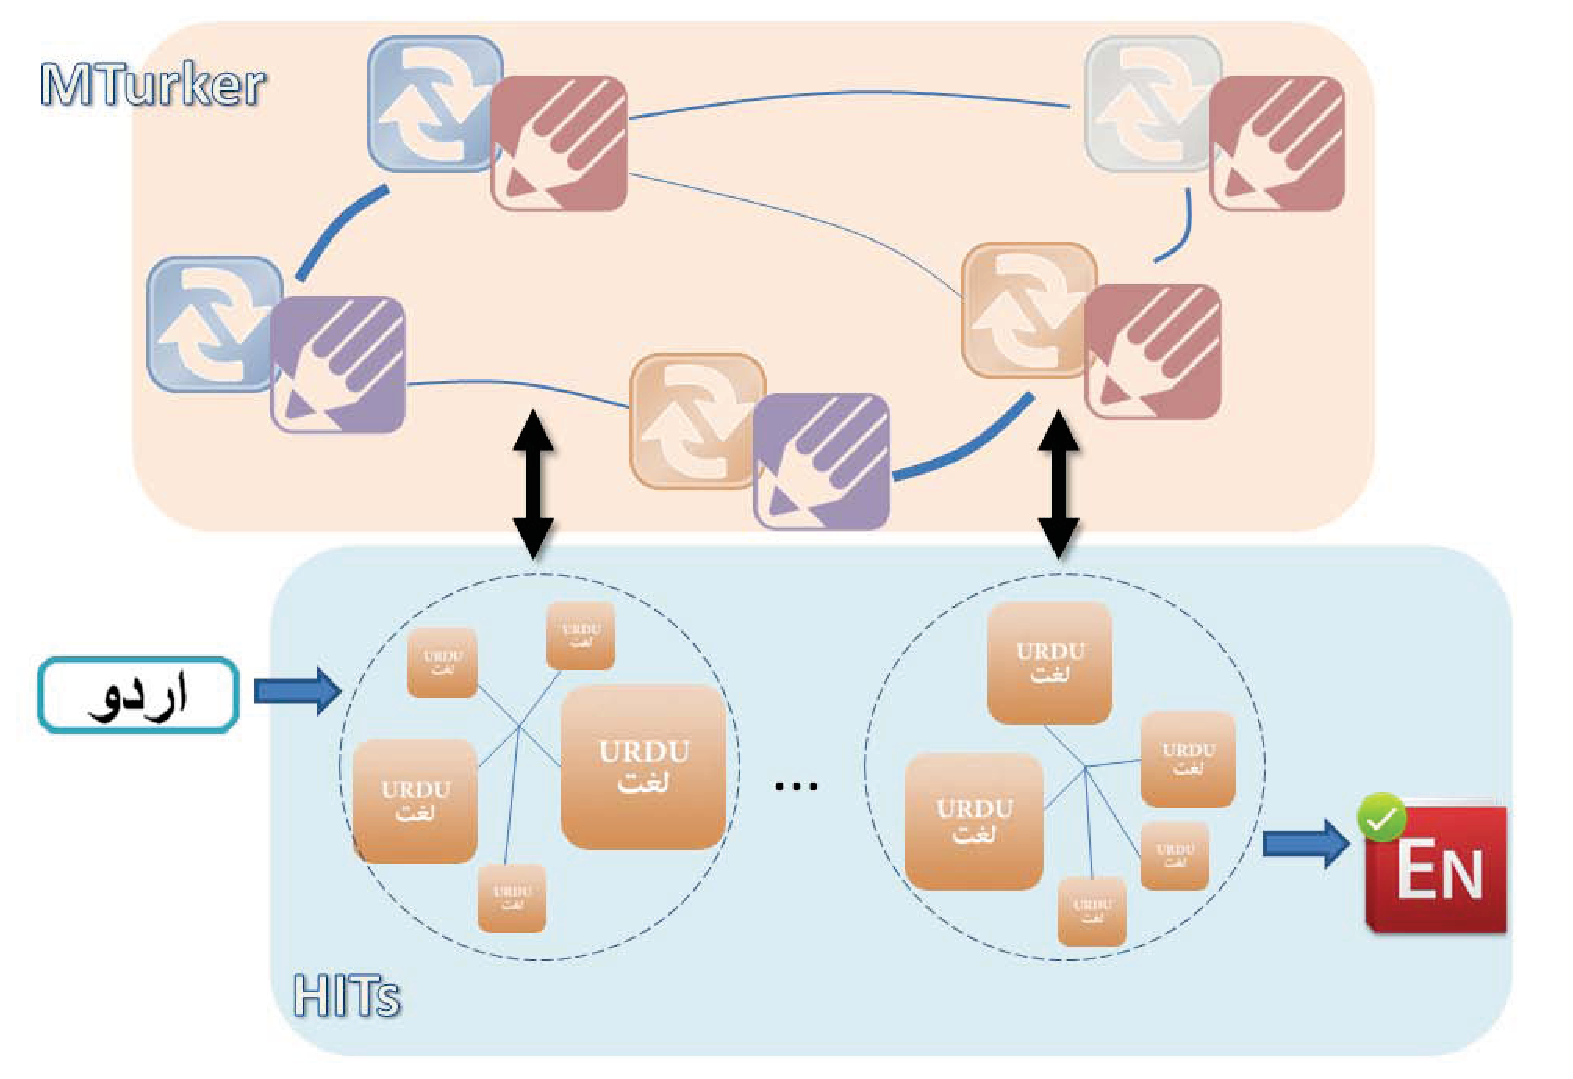
\includegraphics[width=0.68\textwidth]{framework}
  \caption{2-step collaborative crowdsourcing translation model based on graph ranking framework including three sub-networks. The undirected links between users denotes \textit{translation-editing} collaboration. The undirected links between candidate translations indicate lexical similarity between candidates. A bipartite graph ties candidate and Turker networks together by authorship (to make the figure clearer, some linkage is omitted). A dashed circle indicates the group of candidate translations for a single source sentence to translate.}
  \label{frame}
\end{figure*}

\subsection{Inter-Graph Ranking}

The framework includes three random walks, one on $G_T$, one on $G_C$ and one on $G_{TC}$. A random walk on a graph is a Markov chain, its states being the vertices of the graph. It can be described by a stochastic square matrix, where the dimension is the number of vertices in the graph, and the entries describe the transition probabilities from one vertex to the next. The mutual reinforcement framework couples the two random walks on $G_T$ and $G_C$ that rank candidates and Turkers in isolation. The ranking method allows us to obtain a global ranking by taking into account the intra-/inter-component dependencies. In the following sections, we describe how we obtain the rankings on $G_T$ and $G_C$, and then move on to discuss how the two are coupled.

Our algorithm aims to capture the following intuitions. A candidate is important if 1) it is similar to many of the other proposed candidates and 2) it is authored by better qualified translators and/or post-editors. Analogously, a translator/editor pair is believed to be better qualified if 1) the editor is collaborating with a good translator and vice versa and 2) the pair has authored important candidates. This ranking schema is actually a reinforced process across the heterogeneous graphs. We use two vectors $\textbf{c}=[\pi(c)]_{|c| \times 1}$ and $\textbf{t}=[\pi(t)]_{|t| \times 1}$ to denote the saliency scores $\pi(.)$ of candidates and Turker pairs. The above-mentioned intuitions can be formulated as follows:

$\bullet$ \textbf{Homogeneity.} We use adjacency matrix $[M]_{|\textbf{c}|\times |\textbf{c}|}$ to describe the homogeneous affinity between candidates and $[N]_{|\textbf{t}| \times |\textbf{t}|}$ to describe the affinity between Turkers.
\begin{equation}
\textbf{c} \propto {M}^{T} \textbf{c}, \qquad \textbf{t} \propto {N}^{T} \textbf{t}
\end{equation}

where $c=|V_C|$ is the number of vertices in the candidate graph and $t=|V_T|$ is the number of vertices in the Turker graph. The adjacency matrix $[M]$ denotes the transition probabilities between candidates, and analogously matrix $[N]$ denotes the affinity between Turker collaboration pairs.

$\bullet$ \textbf{Heterogeneity.} We use an adjacency matrix $[\hat{W}]_{|\textbf{c}| \times |\textbf{t}|}$ and $[\bar{W}]_{|\textbf{t}|\times |\textbf{c}|}$ to describe the authorship between the output candidate and the producer Turker pair from both of the candidate-to-Turker and Turker-to-candidate perspectives.
\begin{equation}
\textbf{c} \propto \hat{W}^{T} \textbf{t}, \qquad \textbf{t} \propto \bar{W}^{T} \textbf{c}
\end{equation}

All affinity matrices will be defined in the next section. By fusing the above equations, we can have the following iterative calculation in matrix forms. For numerical computation of the saliency scores, the initial scores of all sentences and Turkers are set to 1 and the following two steps are alternated until convergence to select the best candidate. 

\textbf{Step 1}: compute the saliency scores of candidates, and then normalize using $\ell$-1 norm.
\begin{equation}
\begin{aligned}
\textbf{c}^{(n)}&=(1-\lambda) {M}^{T}\textbf{c}^{(n-1)}+\lambda \hat{W}\textbf{t}^{(n-1)}\\
\textbf{c}^{(n)}&=\textbf{c}^{(n)}/||\textbf{c}^{(n)}||_1
\end{aligned}
\end{equation}

\textbf{Step 2}: compute the saliency scores of Turker pairs, and then normalize using $\ell$-1 norm.
\begin{equation}
\begin{aligned}
\textbf{t}^{(n)}&=(1-\lambda) {N}^{T}\textbf{t}^{(n-1)}+\lambda \bar{W}\textbf{c}^{(n-1)}\\
\textbf{t}^{(n)}&=\textbf{t}^{(n)}/||\textbf{t}^{(n)}||_1
\end{aligned}
\end{equation} where $\lambda$ specifies the relative contributions to the saliency score trade-off between the homogeneous affinity and the heterogeneous affinity. In order to guarantee the convergence of the iterative form, we must force the transition matrix to be stochastic and irreducible. To this end, we must make the \textbf{c} and \textbf{t} \textit{column stochastic} \cite{a20}. \textbf{c} and \textbf{t} are therefore normalized after each iteration of Equation (4) and (5).

\subsection{Intra-Graph Ranking}
The standard PageRank algorithm starts from an arbitrary node and randomly selects to either follow a random out-going edge (considering the weighted transition matrix) or to jump to a random node (treating all nodes with equal probability). 

%From Ellie - I am not sure what this sentence is referring to, or why it is included ??
%Note that the generated candidate could be pre-judged to be of different linguistics qualities \cite{a14,zaidan-callisonburch:2011:ACL-HLT2011a}, we can incorporate textual quality as the transitional prior. However, since linguistics quality is not the focus of this work, we simplify the study by starting with the standard ranking. 

%the general textual quality judgement described in \cite{zaidan-callisonburch:2011:ACL-HLT2011a}. We use the following criteria as indicators of the quality of the generations:
%
%\textbf{Sentence-Level}. The first set of features attempt to discriminate good English sentences from bad ones before the graph ranking process.
%
%$\bullet$ Language model features: each sentence is assigned with a log probability and per-word perplexity score, using a 5-gram language model trained on the English Gigaword corpus.
%
%$\bullet$ Sentence length features: a good translation tends to be comparable in length to the source sentence, whereas an overly short or long translation is probably bad. We add two features that are the ratios of the two lengths (one penalizes short sentences and one penalizes long ones).
%
%$\bullet$ Web n-gram match percentage: we assign a score to each sentence based on the percentage of the n-grams (up to length 5) in the translation that exist in the Google N-Gram Database.
%
%$\bullet$ Web n-gram geometric average: we calculate the average over the different n-gram match percentages (similar to the way BLEU is computed). We add three features corresponding to max n-gram lengths of 3, 4, and 5.
%
%\textbf{Turker-Level.} We add Turker-level features that evaluate a translation based on the generators who provided the translation and post-editing.
%
%$\bullet$ Aggregate features: for each sentence-level feature above, we have a corresponding feature computed over all of that worker's translations. The score for the working pair is calculated as the 1) average, 2) maximum and 3) minimum score of both Turkers.
%
%$\bullet$ Activity features: we also investigate the total number of productions and the ratio of the high quality productions from the working pair.
%
%We could also use the features such as location information or language ability information. Since currently these information is not well certified, we temporarily leave it out of the Turker-Level feature now.
%
%After calculation of all features, we sort out an overall score to measure the linguistics and Turker quality based on regression when apply the linear combination measurement in \cite{zaidan-callisonburch:2011:ACL-HLT2011a}, the quality scores are denoted as $\textbf{h}_0$ for HIT and $\textbf{t}_0$ for Turker pairs.

In a simple random walk, it is assumed that all nodes in the transitional matrix are equi-probable before the walk starts. Then \textbf{c} and \textbf{t} are calculated as:
\begin{equation}
\textbf{c}=\mu M^{T}\textbf{c} + (1-\mu) \frac{\textbf{1}}{|V_C|}
\end{equation}

and
\begin{equation}
\textbf{t}=\mu N^{T}\textbf{t} + (1-\mu) \frac{\textbf{1}}{|V_T|}
\end{equation} where \textbf{1} is a vector with all elements equaling to 1 and the size is correspondent to the size of $V_C$ or $V_T$. $\mu$ is the damping factor usually set to 0.85, as in the PageRank algorithm.

\subsection{Affinity Matrix Establishment}
\label{affinity}
We introduce the affinity matrix calculation, including homogeneous affinity (i.e., ${M},{N}$) and heterogeneous affinity (i.e., $\hat{W},\bar{W}$).

As discussed, we model the collection of candidates as a weighted undirected graph, $G_C$, in which nodes in the graph represent candidate sentences and edges represent lexical relatedness. We define an edge's weight to be the cosine similarity between the candidates represented by the nodes that it connects. The adjacency matrix M describes such a graph, with each entry corresponding to the weight of an edge.
\begin{equation}
\begin{aligned}
\mathcal{F}&(c_i,c_j)=\frac{c_i \cdot c_j}{||c_i||||c_j||}\\
&M_{ij}=\frac{\mathcal{F}(c_i,c_j)}{\sum_k \mathcal{F}(c_i,c_k)}
\end{aligned}
\end{equation} where $\mathcal{F}(.)$ is the cosine similarity and $c$ is a term vector corresponding to a candidate. We treat a candidate as a short document and weight each term with \textit{tf.idf} \cite{a16}, where \textit{tf} is the term frequency and \textit{idf} is the inverse document frequency.

The Turker graph, $G_T$, is an undirected graph whose edges represent ``collaboration.'' Formally, let $t_i$ and $t_j$ be two translator/editor pairs; we say that pair $t_i$ ``collaborates with'' pair $t_j$ (and therefore, there is an edge between $t_i$ and $t_j$) if $t_i$ and $t_j$ share either a translator or an editor (or share both a translator and an editor). Let the function $\mathcal{I}(t_i,t_j)$ denote the number of ``collaborations'' ($\#col$) between $t_i$ and $t_j$. 
\begin{equation}
\begin{aligned}
\mathcal{I}(t_i,t_j)&=
\begin{cases}
\#col &(e_{ij} \in E_T) \\
0 &\text{otherwise}
\end{cases}, \\
\end{aligned}
\end{equation}

Then the adjacency matrix N is then defined as

\begin{equation}
\begin{aligned}
N_{ij}&=\frac{\mathcal{I}(t_i,t_j)}{\sum_k \mathcal{I}(t_i,t_k)}
\end{aligned}
\end{equation}

In the bipartite candidate-Turker graph $G_{TC}$, the entry $E_{TC}(i, j)$ is an indicator function denoting whether the candidate $c_i$ is generated by $t_j$:
\begin{equation}
\mathcal{A}(c_i,t_j)=
\begin{cases}
1 &(e_{ij} \in E_{TC}) \\
0 &\text{otherwise}
\end{cases}
\end{equation}

Through $E_{TC}$ we define the weight matrices $\bar{W}_{ij}$ and $\hat{W}_{ij}$, containing the conditional probabilities of transitions from $c_i$ to $t_j$ and vice versa:
\begin{equation}
\begin{aligned}
&\bar{W}_{ij}=\frac{\mathcal{A}(c_i,t_j)}{\sum_k \mathcal{A}(c_i,t_k)},\\
&\hat{W}_{ij}=\frac{\mathcal{A}(c_i,t_j)}{\sum_k \mathcal{A}(c_k,t_j)}
\end{aligned}
\end{equation}

\section{Evaluation}

We are interested in testing our random walk method, which incorporates information from both the candidate translations and from the Turkers. We want to test two versions of our proposed collaborative co-ranking method: 1) based on the unedited translations only and 2) based on the edited sentences after translator/editor collaborations. 

\paragraph{Metric} Since we have four professional translation sets, we can calculate the Bilingual Evaluation Understudy (BLEU) score \cite{a17} for one professional translator (P1) using the other three (P2,3,4) as a reference set. We repeat the process four times, scoring each professional translator against the others, to calculate the expected range of professional quality translation. In the following sections, we evaluate each of our methods by calculating BLEU scores against the same four sets of three reference translations. Therefore, each number reported in our experimental results is an average of four numbers, corresponding to the four possible ways of choosing 3 of the 4 reference sets. This allows us to compare the BLEU score achieved by our methods against the BLEU scores achievable by professional translators.

%We also evaluate translation quality by using reference sets to score various submissions to the NIST MT evaluation. Specifically, we measure the correlation (using Pearson r) between BLEU scores of MT systems measured against non-professional translations, and BLEU scores measured against professional translations. Since the main purpose of the NIST dataset was to compare MT systems against each other, this is a more direct fitness-for-task measure. We chose the middle 6 systems (in terms of performance) submitted to the NIST evaluation, out of 12, as those systems were fairly close to each other, with less than 2 BLEU points separating them.



\begin{table}[t]
\centering
\begin{tabular}{|c||c|} \hline
Reference (Avg.)   &42.51        \\   \hline 
Oracle (Seg-Trans)  &44.92	          \\  \hline
Oracle (Seg-Tran+Edit)  &48.44	          \\  \hline
Oracle (Turker-Trans)    &38.66 \\ \hline
Oracle (Turker-Tran+Edit)    &39.16 \\ \hline \hline
Random &30.52  	           \\ \hline 
Lowest TER   &35.78  \\  \hline
Graph Ranking (Trans)   &38.88  \\  \hline
Graph Ranking (Tran+Edit)   &\textbf{41.43}  \\  \hline
\end{tabular}
\caption{Overall BLEU performance for all methods. The highlighted yellow bars indicate methods based on both candidate and Turker information, with and without post-editing.}
\label{summary-results}
\end{table}

\paragraph{Baselines}

As a naive baseline, we choose one candidate translation at random for each input Urdu sentence. To establish an upper bound for our methods, and to determine if there exist high-quality Turker translations at all, we compute four oracle scores. The first oracle operates at the segment level on the sentences produced by translators only: for each source segment, we choose from the translations the one that scores highest (in terms of BLEU) against the reference sentences. The second oracle is applied similarly, but chooses from the candidates produced by the collaboration of translator/post-editor pairs. The third oracle operates at the worker level: for each source segment, we choose from the translations the one provided by the worker whose translations (over all sentences) score the highest on average. The fourth oracle also operates at the worker level, but selects from sentences produced by translator/post-editor collaborations. These oracle methods represent ideal solutions under our scenario. We also examine two voting-inspired methods. The first method selects the translation with the minimum average TER \cite{a18} against the other translations; intuitively, this would represent the ``consensus'' translation. The second method selects the translation generated by the Turker who, on average, provides translations with the minimum average TER.



\paragraph{Results}

A summary of our results in given in Table \ref{summary-results}. As expected, random selection yields bad performance, with a BLEU score of 30.52. The oracles indicate that there is usually an acceptable translation from the Turkers for any given sentence. Since the oracles select from a small group of only 4 translations per source segment, they are not overly optimistic, and rather reflect the true potential of the collected translations. On average, the reference translations give a score of 42.38. To put this in perspective, the output of a state-of-the-art machine translation system (the syntax-based variant of Joshua) achieves a score of 26.91, which is reported in \cite{zaidan-callisonburch:2011:ACL-HLT2011a}. The approach which selects the translations with the minimum average TER \cite{a18} against the other three translations (the ``consensus'' translation) achieves BLEU scores of 35.78. %The second method selects the translation from the Turkers with the minimum average TER based on all their translations. These approaches achieve BLEU scores of 34.41 and 33.28, respectively.

Using the raw translations without post-editing, our graph-based ranking method achieves a BLEU score of  38.89, compared to \newcite{zaidan-callisonburch:2011:ACL-HLT2011a}' s reported score of 28.13, which they achieved using a linear feature-based classification. Their linear classifier achieved a reported score of 39.06\footnote{Note that the data we used in our experiments are slightly different, by discarding nearly 100 NULL sentences in the raw data. We do not re-implement this baseline but report the results from the paper directly. According to our experiments, most of the results generated by baselines and oracles are very close to the previously reported values.} when combining information from both translators and editors. In contrast, our proposed graph-based ranking framework achieves a score of 41.43 when using the same information. This boost in BLEU score confirms our intuition that the hidden collaboration networks between candidate translations and transltor/editor pairs are indeed useful.

\paragraph{Parameter Tuning}

\begin{figure}[t]
  \centering
  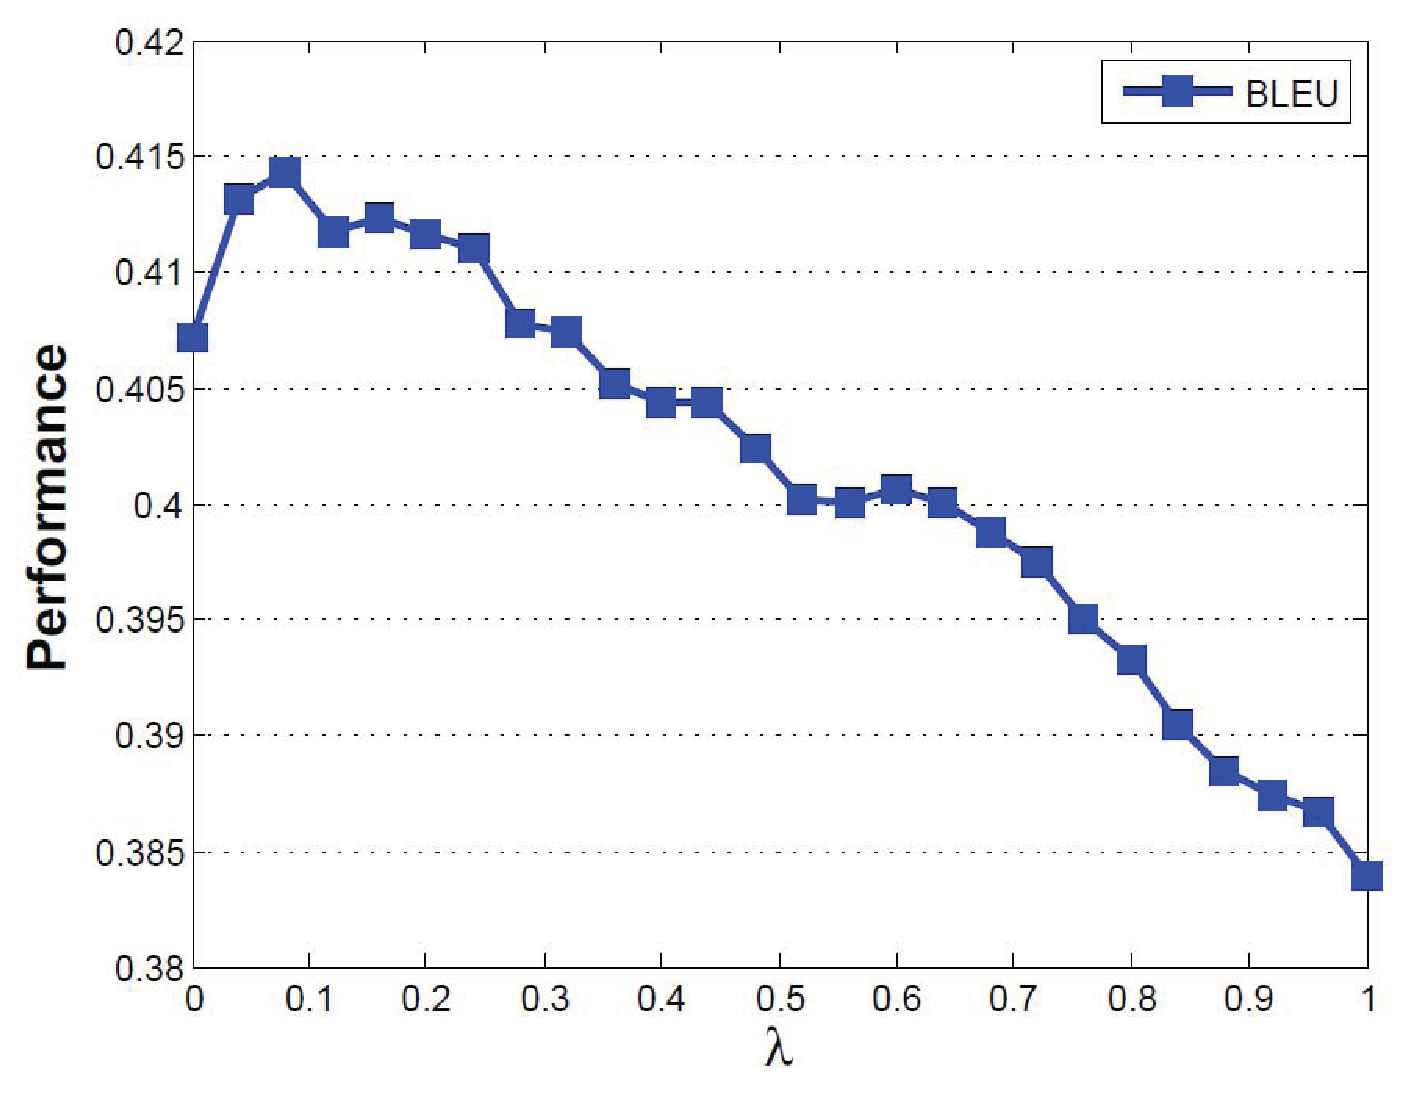
\includegraphics[width=0.48\textwidth]{parameters}
  \caption{Effect of candidate-Turker coupling ($\lambda$) on BLEU score.}
  \label{lambda}
\end{figure}

There are two parameters in our experimental setups: $\mu$ controls the probability of starting a new random walk and $\lambda$ controls the coupling between the candidate and Turker sub-graphs. We set the damping factor $\mu$ to 0.85, following the standard PageRank paradigm. In order to determine a value for $\lambda$, we used the average BLEU, computed against the professional reference translations, as a tuning metric. We experimented with values of $\lambda$ ranging from 0 to 1, with a step size of 0.05 (Figure \ref{lambda}). Small $\lambda$ values place little emphasis on the candidate/Turker coupling, whereas larger values rely more heavily on the co-ranking. Overall, we observed better performance with values within the range of 0.05-0.15. This suggests that both sources of information-- the candidate itself and its authors-- are important for the crowdsourcing translation task. In all of our reported results, we used the $\lambda$ = 0.1.

\paragraph{Analysis}
We examine the relative contribution of each component of our approach on the overall performance. We first examine the centroid-based ranking on the candidate sub-graph ($G_C$) alone to see the effect of voting among translated sentences; we denote this strategy as \textit{plain ranking}. Then we incorporate the standard random walk on the Turker graph ($G_T$) to include the structural information but without yet including any collaboration information; that is, we incorporate information from $G_T$ and $G_C$ without including edges linking the two together. The co-ranking paradigm is exactly the same as the framework described in Section 3.2, but with simplified structures.

Finally, we examine the two-step collaboration based candidate-Turker graph using several variations on edge establishment. As before, the nodes are the translator/post-editor working pairs. We investigate three settings in which 1) edges connect two nodes when they share only a translator, 2) edges connect two nodes when they share only a post-editor, and 3) edges connect two nodes when they share either a translator or a post-editor. These results are summarized in Table \ref{component-variation}. 

\begin{table}[t]
\centering
\begin{tabular}{|c||c|} \hline
Plain ranking   &38.89        \\   \hline \hline
w/o collaboration &38.88  	           \\ \hline \hline
Shared translator  &41.38	          \\  \hline
Shared post-editor    &41.29 \\ \hline
Shared Turker   &\textbf{41.43}  \\  \hline
\end{tabular}
\caption{Variations of all component settings.}
\label{component-variation}
\end{table}

Interestingly, we observe that when modeling the linkage between the collaboration pairs, connecting Turker pairs which share either a translator or the post-editor achieves better performance than connecting pairs that share only translators or connecting pairs which share only editors. This result supports the intuition that a denser collaboration matrix will help propagate saliency to good translators/post-editors and hence provides better predictions for candidate quality.

%\section{Related Work}
%Extraneous data source could always be a supplement to improve MT models so that they are better suited to the low resource setting \cite{a21,a22}. Transfer learning based models, or designing models that are capable of learning translations from monolingual corpora \cite{a23,a24}.
%
%Dawid and Skene \shortcite{a1} investigated filtering annotations using the EM algorithm, estimating annotator-specific error rates in the context of patient medical records. Snow et al. \shortcite{a2} were among the first to use MTurk to obtain data for several NLP tasks, such as textual entailment and word sense disambiguation. Their approach, based on majority voting, had a component for annotator bias correction. They showed that for such tasks, a few non-expert labels usually suffice.
%
%Whitehill et al. \shortcite{a3} proposed a probabilistic model to filter labels from non-experts, in the context of an image labeling task. Their system generatively models image difficulty, as well as noisy, even adversarial, annotators. They apply their method to simulated labels rather than real-life labels.
%
%Callison-Burch \shortcite{a4} proposed several ways to evaluate MT output on MTurk. One such method was to collect reference translations to score MT output. It was only a pilot study (50 sentences in each of several languages), but it showed the possibility of obtaining high-quality translations from non-professionals. As a followup, Bloodgood and Callison-Burch \shortcite{a5} solicited a single translation of the NIST Urdu-to-English dataset we used. Their evaluation was similar to our correlation experiments, examining how well the collected translations agreed with the professional translations when evaluating three MT systems.
%
%That paper appeared in a NAACL 2010 workshop organized by Callison-Burch and Dredze \shortcite{a6}, focusing on MTurk as a source of data for speech and language tasks. Two relevant papers from that workshop were by Ambati and Vogel \shortcite{a7}, focusing on the design of the translation HIT, and by Irvine and Klementiev \shortcite{a8}, who created translation lexicons between English and 42 rare languages.
%
%Resnik et al. \shortcite{a9} explore a very interesting way of creating translations on MTurk, relying only on monolingual speakers. Speakers of the target language iteratively identified problems in machine translation output, and speakers of the source language paraphrased the corresponding source portion. The paraphrased source would then be retranslated to produce a different translation, hopefully more coherent than the original.

\section{Conclusion}
We have proposed an algorithm for using a two-step collaboration between non-professional translators and post-editors to obtain professional-quality translations. Our method, based on a co-ranking model,  selects the best crowdsourced translation from a set of candidates, and is capable of selecting translations which near professional quality.

Crowdsourcing can play a pivotal role in future efforts to create parallel translation datasets. In addition to its benefits of cost and scalability, crowdsourcing provides access to languages that currently fall outside the scope of statistical machine translation research. In future work on crowdsourced translation, further benefits in quality improvement and cost reduction could stem from 1) building ground truth data sets based on high-quality Turkers' translations and 2) identifying when sufficient data has been collected for a given input, to avoid soliciting unnecessary redundant translations.

\section*{Acknowledgements}
This material is based on research sponsored by a DARPA Computer Science Study Panel phase 3 award entitled ``Crowdsourcing Translation'' (contract D12PC00368). The views and conclusions contained in this publication are those of the authors and should not be interpreted as representing official policies or endorsements by DARPA or the U.S. Government. This research was supported by the Johns Hopkins University Human Language Technology Center of Excellence and through gifts from Microsoft, Google and Facebook.

\bibliographystyle{acl2014}
\bibliography{acltranslation}




%The acknowledgments should go immediately before the references.  Do
%not number the acknowledgments section. Do not include this section
%when submitting your paper for review.





\end{document}
